\documentclass[lettersize,journal]{IEEEtran}
\usepackage{iftex}
\ifXeTeX\usepackage{fontspec}\setmainfont{texgyretermes}[Extension=.otf,UprightFont=*-regular,BoldFont=*-bold,ItalicFont=*-italic,BoldItalicFont=*-bolditalic]\fi
\usepackage{amsmath,amsfonts}
\usepackage{array}
\usepackage{booktabs}
\usepackage[caption=false,font=normalsize,labelfont=sf,textfont=sf]{subfig}
\usepackage{textcomp}
\usepackage{stfloats}
\usepackage{url}
\usepackage{verbatim}
\usepackage{graphicx}
\usepackage{cite}
\usepackage{xcolor}
\hyphenation{op-tical net-works semi-conduc-tor IEEE-Xplore}
\newcommand{\ellv}{\ell}

\begin{document}

\title{Auditing and Repairing the Missing-Modality Generation Module of Multimodal Prompt Learning: Length-Bound Parameters, a Dead Prompt, and Real CLIP Features}

\author{Sujal Som (B24DS032), Ashish Kumar Dash (B24CS009), Tanmay Jaiswal (B24DS033)\\
CS550 Machine Learning, IIT Bhilai}

\maketitle

\begin{abstract}
Multimodal Prompt Learning with Missing Modalities (MPLMM, ACL 2024) freezes a pretrained Multimodal Transformer and learns three small prompt types plus a ``lightweight'' generation module that synthesises absent modalities. Its authors state that the module may fail on raw features, which they expect to be less correlated across modalities. We audited the released code and tested that limitation on CMU-MOSI.
\emph{Audit.} One of the three prompt types is zero-initialised on both sides of a bilinear product, so it never receives gradient. It is all-zero in 55 of 55 trained runs, and the paper's Table~3 ablation cannot be reproduced from the released code; re-initialising its four tensors to $\mathcal{N}(0,0.02)$ makes all four train. The released configuration reports the validation split instead of the test split, applies modality dropout to the evaluation splits, selects checkpoints on loss and stops early: it gives 57.55\% against the reported 72.14\%, and a corrected schedule recovers 67.51\%. The code does not install from its stated requirements and needs two patches to load its own checkpoints on current PyTorch. The module's time-mixing layer is dense over \emph{time}, so its size grows with sequence length, reaching 1,115,666 trainable parameters at native length, 104\% of the frozen backbone. The upstream training loop and our fork's loop differ by 7.6 points on the same $\ell=50$ cell, so we never compare numbers across loops.
\emph{Repair.} A length-invariant cross-attention operator matches the dense module at every length we tested, and is equivalent within the pre-registered $\pm$2-point margin at native length with 5.86$\times$ fewer parameters (pooled over two machines, TOST $p=0.033$). Deleting the learned time-mixing layer altogether costs no detectable accuracy at $\ell=200$. The logged generation-fidelity metric mostly measures padding layout.
\emph{Real foundation features.} We extracted CLIP ViT-B/32 features from all 2,199 raw MOSI clips. Swapping Facet for real CLIP vision causes no detectable accuracy change, and real CLIP vision is not less correlated with the text than Facet once speaker identity is removed. A label-aware projection prescribed by our own proposal turns out to be an invalid control: it memorises training-speaker sentiment.
\end{abstract}

\begin{IEEEkeywords}
Multimodal sentiment analysis, missing modalities, prompt learning, reproducibility, parameter efficiency, CLIP, centered kernel alignment.
\end{IEEEkeywords}

\section{Introduction}
\IEEEPARstart{M}{ultimodal} sentiment analysis predicts the sentiment of a short video clip from three co-occurring streams: the transcript, the voice and the face. In deployment, streams go missing: a microphone clips, a face leaves the frame, a transcript fails. Models trained on complete triplets then degrade. MPLMM~\cite{guo2024mplmm} avoids elaborate reconstruction networks. It freezes a pretrained Multimodal Transformer (MulT)~\cite{tsai2019mult} and learns only three small prompt types: a generative prompt, a missing-signal prompt and a missing-type prompt. A deliberately simple generation module fills in absent modalities. The paper reports 72.14\% average binary accuracy over six missing-modality cases on CMU-MOSI~\cite{zadeh2016mosi}, against 70.84\% for MMIN~\cite{zhao2021mmin}.

The authors name one limitation themselves: because the generation module is simple, ``the performance of the model could degrade if we use raw features which are much more complicated and have weaker correlation between modalities than extracted features'', and they leave this to future work~\cite{guo2024mplmm}. Our project takes that limitation as its target. Reading the released implementation, we found a property the paper does not report: the module's main operator is a dense linear map over \emph{time}, so its parameter count is bound to the sequence length. This predicts a second failure mode, driven by length rather than by inter-modal correlation.

We asked three questions, following our proposal (SOP):
\begin{itemize}
\item \textbf{Q1 (structural).} How do the module's parameters and inductive bias scale with sequence length?
\item \textbf{Q2 (diagnostic).} Does performance degrade with sequence length, feature dimensionality or inter-modal correlation?
\item \textbf{Q3 (repair).} Can a length-invariant operator replace the dense map without losing accuracy?
\end{itemize}

\textbf{Contributions.}
\begin{enumerate}
\item \textbf{Code audit.} We locate each fault in the released code at a line number (Table~\ref{tab:faults}): a prompt type that never trains, with a verified one-line repair; four training and evaluation faults that together cost 14.59 points; an undisclosed length scaling that makes the module larger than the backbone at native length; a configuration flag whose two branches are identical; and five environment blockers (Section~\ref{sec:audit}).
\item \textbf{Two training loops.} The upstream loop is bit-reproducible per machine and our fork's loop is not, and the two differ by 7.6 points on the same cell. We quantify this and keep every comparison inside one loop (Section~\ref{sec:loops}).
\item \textbf{Repair.} A length-invariant operator matches the dense module across a four-rung length ladder, and is statistically equivalent at native length at 5.86$\times$ fewer parameters, replicated on two machines (Section~\ref{sec:results}).
\item \textbf{Ablation.} Removing the learned time-mixing parameters entirely costs no detectable accuracy on the paper's features. The logged fidelity metric fails a negative control (Section~\ref{sec:ablation}).
\item \textbf{Real foundation features.} We built and verified a CLIP extractor on the raw MOSI video. The degradation the authors predict does not appear for vision, and the premise behind it, weaker inter-modal correlation, does not hold for vision (Section~\ref{sec:clip}).
\item \textbf{Negative results, reported.} Our own robustness prediction was wrong. A synthetic stand-in for foundation features was mislabelled. The label-aware control our proposal prescribed is invalid on speaker-independent splits.
\end{enumerate}

\subsection{Project details and team contributions}
\textbf{Criterion followed:} the code is available, so we address a stated limitation and propose a solution. Target paper: Guo \emph{et al.}, ACL 2024~\cite{guo2024mplmm}; code: \url{https://github.com/zrguo/MPLMM}.
\begin{itemize}
\item \textbf{Tanmay Jaiswal} (B24DS033, tanmay@iitbhilai.ac.in), feature pipeline and data:
  \begin{itemize}
  \item MOSEI backbone pre-training;
  \item the pooling-based sequence-length ladder (resampler with native-length identity check);
  \item the 200-epoch launcher.
  \end{itemize}
  The SOP also assigned him the CLIP extractor and merge utility; see the next entry for who built them.
\item \textbf{Sujal Som} (B24DS032, sujals@iitbhilai.ac.in), model and training:
  \begin{itemize}
  \item baseline reproduction runs;
  \item the length-invariant operator (\texttt{lenmod/operator.py});
  \item the forward hooks for fidelity scoring (\texttt{lenmod/hooks.py});
  \item the 200-epoch training runs and operator ablations (arms C/D);
  \item the CLIP extractor and merge utility code.
  \end{itemize}
\item \textbf{Ashish Kumar Dash} (B24CS009, ashishkd@iitbhilai.ac.in), evaluation and analysis:
  \begin{itemize}
  \item the code audit: parameter audit, inductive-bias probes, the dead-prompt proof, and diagnosis of the evaluation-split fault;
  \item the claims ledger and statistical protocol;
  \item the fidelity audit (\texttt{tools/fidelity\_audit.py}) and inter-modal CKA (\texttt{tools/intermodal\_cka.py});
  \item the real-data CLIP run: extractor hardening, verification, speaker controls and the PCA control;
  \item the figures and this report.
  \end{itemize}
\end{itemize}

\section{Related Work}
\textbf{Missing-modality learning.} Imagination and reconstruction approaches learn to regenerate absent streams. MMIN~\cite{zhao2021mmin}, for example, uses cascaded residual autoencoders. These need sizeable reconstruction networks. Prompt-based alternatives began with missing-aware prompts for vision--language recognition~\cite{lee2023missingprompts}, which build on prefix tuning~\cite{li2021prefix} and visual prompt tuning~\cite{jia2022vpt}. MPLMM~\cite{guo2024mplmm} adds a generation module, a real-versus-generated signalling prompt, and a compositional missing-type prompt that scales linearly in the number of modalities. A recent preprint questions whether generating missing modalities is needed at all, and evaluates before generating~\cite{evalbeforegen2026}. Our ablation in Section~\ref{sec:ablation} is a direct, controlled test of that question for MPLMM.

\textbf{Features for multimodal sentiment.} The CMU-MOSI and CMU-MOSEI~\cite{zadeh2018mosei} benchmarks are usually consumed as pre-extracted features: GloVe word vectors~\cite{pennington2014glove}, COVAREP acoustic descriptors~\cite{degottex2014covarep}, and Facet facial action units~\cite{ekman1978facs}. Both non-text streams are hand-designed to track affect, which is the basis for the authors' expectation that raw or foundation-model features (wav2vec~2.0~\cite{baevski2020wav2vec}, CLIP~\cite{radford2021clip}) would be harder. End-to-end models on raw inputs exist~\cite{dai2021sparse}. Toolkits such as MMSA and MMSA-FET~\cite{mao2022msena} distribute features and raw clips, but MMSA-FET has no CLIP extractor.

\textbf{Representation similarity and equivalence testing.} We measure generation fidelity and inter-modal coupling with linear centered kernel alignment (CKA)~\cite{kornblith2019cka}. We state equivalence only with two one-sided tests (TOST)~\cite{schuirmann1987tost} against a pre-registered margin.

\section{Proposed Methodology}
\subsection{The generation module as released}
Fig.~\ref{fig:pipeline} shows the language-missing case. Two pointwise convolutions (\texttt{a2l}, \texttt{v2l}) mix channels at each time step. Their outputs are concatenated along \emph{time} with a generative prompt of length $\ell_p=16$. A transpose then moves the time axis into the channel slot of a \texttt{Conv1d(kernel\_size=1)} layer (\texttt{l\_avp}). That layer is therefore a dense, position-indexed linear map over time: every output position draws on every input position, with no weight sharing, locality or translation-equivariance. A learned missing-signal prompt is added (an addition, not a residual connection), and the result enters the frozen MulT backbone. A missing-type prompt is prepended for every sample. For a time-mixer with output length $\ell_{out}$ and total input length $\ell_{in}=\ell_p+\sum\ell_{src}$, the parameter count is
\begin{equation}
P_{\text{dense}} = \ell_{out}\,\ell_{in} + \ell_{out}. \label{eq:params}
\end{equation}
Nine such layers exist: three two-source generators and six single-source generators. Each is bilinear in output and input length, hence quadratic when all modalities lengthen together.

\begin{figure*}[!t]
\centering
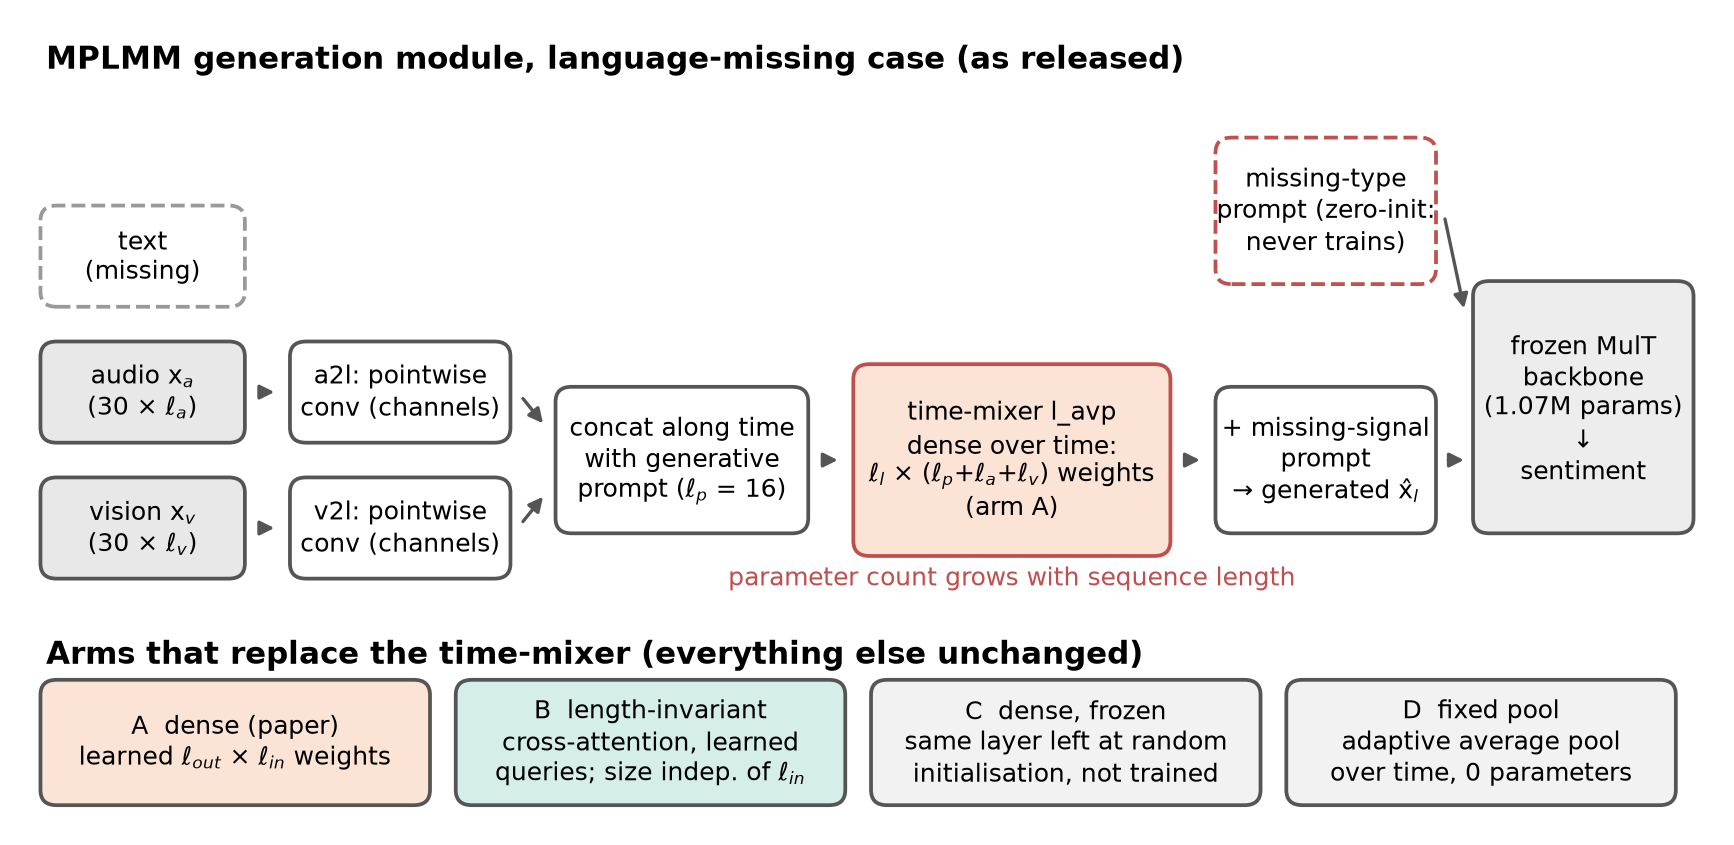
\includegraphics[width=0.92\textwidth]{fig_pipeline}
\caption{The MPLMM generation module (language-missing case, as released) and the four arms that replace its time-mixing layer. Arms differ only in the time-mixer; prompts, channel mixers and the frozen MulT backbone are identical. The missing-type prompt is zero-initialised in a bilinear product and never trains (Section~\ref{sec:audit}).}
\label{fig:pipeline}
\end{figure*}

\subsection{Audit method}
Every structural claim is checked by two independent routes before it is reported.
\begin{itemize}
\item \textbf{Parameter counts.} \texttt{tools/count\_params.py} computes each count twice, by instantiating the real \texttt{PromptModel} and by the closed form of Eq.~(\ref{eq:params}), and asserts that the two agree.
\item \textbf{Inductive bias.} We perturb single time positions and single feature channels, and measure the diagonal mass of trained weights against chance.
\item \textbf{Trainability of the missing-type prompt.} Five routes: hand derivation, a standalone reimplementation, a state-dict check, functional perturbation, and Adam at learning rate~1.
\item \textbf{Reproduction.} The released configuration is compared against a corrected schedule, with each fault located at a line number.
\end{itemize}

\subsection{The length-invariant operator (arm B)}
We replace each of the nine time-mixers with cross-attention from a fixed set of learned queries to all available input tokens:
\begin{equation}
\hat{x} = \mathrm{GELU}\big(\mathrm{MHA}(Q, X, X)\big),\qquad Q\in\mathbb{R}^{\ell_q\times d_p},
\end{equation}
with $\ell_q=50$ learned queries of width $d_p=30$ and two attention heads. If $\ell_{out}\neq\ell_q$, the queries are linearly interpolated along time. The operator's own parameters do not depend on $\ell_{in}$. The missing-signal prompts and missing-type coupling stay length-dependent, so total trainable parameters still grow, linearly. Only the operator is replaced; everything else in the model is unchanged.

\subsection{Operator ablations (arms C and D)}
Two arms separate ``a dense map is needed'' from ``these parameters are needed''.
\begin{itemize}
\item \textbf{Arm C} keeps the dense time-mixers frozen at their random initialisation, as a negative control. A fingerprint check asserts the weights are unchanged after backbone transfer.
\item \textbf{Arm D} replaces them with a zero-parameter adaptive average pool over time, followed by the same GELU.
\end{itemize}
Both train exactly the same parameter set (86,491 at $\ell=200$).

\subsection{CLIP visual features from raw video (SOP item 2)}
The extractor loads OpenAI's CLIP ViT-B/32 weights~\cite{radford2021clip}, verified by SHA-256 and frozen. For each segment it:
\begin{enumerate}
\item decodes the clip at 30 fps and native resolution with ffmpeg;
\item applies CLIP's official preprocessing (bicubic shorter-side resize to 224, centre crop, CLIP normalisation);
\item embeds every frame and L2-normalises the embedding.
\end{enumerate}
It raises an error on any time window that decodes to zero frames, and stores the segment IDs alongside the features. Native per-frame embeddings are saved once, and each rung is then derived from them.

To keep layout fixed, the CLIP sequence occupies exactly the word slots that L1's word-aligned Facet features occupy: each clip's frames are split uniformly into $k$ windows, where $k$ is its number of words. The merge utility (SOP item 5) asserts that segment IDs match the reference dataset in order, and refuses inputs produced in synthetic mode. Text (GloVe) and audio (COVAREP) are copied unchanged from the reference file.

\subsection{Fidelity and coupling metrics}
The fork's hooks log linear CKA between generated and real features, flattened over time. Our audit tool rebuilds each checkpoint exactly as training did and must reproduce the stored values (tolerance $5\times10^{-3}$; achieved $\le 1.8\times10^{-7}$) before computing anything new. It adds four corrected measures:
\begin{itemize}
\item CKA on a masked time-mean over real frames only;
\item CKA of generated features against the 0/1 padding mask (a negative control);
\item debiased CKA;
\item \emph{sentiment carried}: the Pearson $r$ between the label and a ridge readout fitted on the \emph{real} modality's training representations and applied to the generated one.
\end{itemize}
Inter-modal coupling is reported as masked, z-scored, clip-level linear CKA against a 200--500-permutation null. Where speaker identity could confound it, we centre each video's features on that video's own mean and permute within videos.

\section{Experimental Setup}
\subsection{Data}
CMU-MOSI~\cite{zadeh2016mosi} has 2,199 opinion segments from 93 speakers, split speaker-independently into 1,284 / 229 / 686 segments (train / valid / test). We use the MulT feature release: GloVe-300 text~\cite{pennington2014glove}, COVAREP-5 audio~\cite{degottex2014covarep} and Facet-20 vision.

\textbf{Length ladder.} The unaligned audio/vision streams are average-pooled with fixed-interval windows to $\ell=50/100/200$; the native rung is 375/500. This holds the extractor fixed and changes only length. Each rung file is checked against \texttt{data/ladder/SHA256SUMS} before use.

\textbf{Aligned L1.} The word-aligned 50-step file. It is 73--74\% zero-padded in every modality.

\textbf{Real CLIP rungs.} Raw clips come from the MMSA release~\cite{mao2022msena}: 2,199 MP4 segments in 93 folders, 518~MB. We checked them against the reference file: all 2,199 IDs matched, there were 0 split mismatches, the maximum label difference was 0.0, and clip durations were within 0.07~s of the reference end$-$start times (61 sampled clips). The official CMU server timed out from our machine. Three CLIP rungs were trained:
\begin{itemize}
\item L2-CLIP: 512-d;
\item L2$'$-CLIP (PCA): PCA to 20-d fitted on train clip means without labels, rescaled to Facet's median row norm;
\item L2$'$-CLIP (PLS): PLS to 20-d fitted on train labels, as the SOP prescribed; built once unscaled and once rescaled.
\end{itemize}
A separate synthetic ``L2'' rung (L1 features rotated into 768/512 dimensions plus orthogonal Gaussian noise) is reported as a noise stressor, not as foundation features (Section~\ref{sec:l2syn}).

\subsection{Training protocol}
All end-term runs share one configuration:
\begin{itemize}
\item one launcher (\texttt{run.py} via \texttt{launch\_e200.py}), with the backbone (\texttt{pretrained/mosei.pt}) frozen;
\item 200 epochs, learning rate $10^{-3}$, batch 16 $\times$ 4 gradient accumulation (effective 64), learning-rate decay patience 30;
\item modality dropout 0.7 during training.
\end{itemize}
Checkpoints are selected on the dropout-0.7 validation split for the length ladder and arms C/D at $\ell=200$. The synthetic-L2 and real-CLIP grids select on complete-data validation (\texttt{--valid\_drop\_rate 0.0}). Each comparison uses one machine, one commit and one protocol. The real-CLIP grid ran entirely at commit \texttt{85eddde}. Our loop does not set \texttt{cudnn.deterministic}, so it is not bit-reproducible even on one machine; upstream \texttt{main.py} sets it and is (Section~\ref{sec:loops}).

\subsection{Metrics and statistics}
\textbf{Primary accuracy.} The \emph{six-case forced mean Acc-2}: each of the six missing-modality cases is forced on all 686 test samples and the six accuracies are averaged. This is the paper-comparable number. Text is present in cases 1, 2 and 5 and absent in cases 0, 3 and 4. Case 6 is complete data.

\textbf{Precision.} One test sample is worth 0.15 points, and the binomial precision floor at $n=686$ is 1.91 points.

\textbf{Tests.} We use 3 seeds per arm, the SOP's pre-registered fallback from 5. With 3 vs 3, the smallest attainable two-sided exact permutation $p$ is 0.10, so large Welch $t$ statistics from 2-degree-of-freedom variance estimates are not reported as small $p$-values. ``No detectable difference'' is never written as ``equivalent''. Equivalence is claimed only with TOST against the SOP's $\pm$2-point margin~\cite{schuirmann1987tost}.

\subsection{Resources}
\begin{itemize}
\item \textbf{Hardware:} one NVIDIA RTX 3060 (12~GB). A 200-epoch run takes about 20--27 minutes at aligned length with two runs sharing the GPU, and about 2~h at native length. The native rung was replicated on a second machine.
\item \textbf{Software:} PyTorch~\cite{paszke2019pytorch}, scikit-learn and ffmpeg.
\item \textbf{Grids:} run by detached, lock-guarded supervisors that restart after a reboot, so that runs do not depend on an open session.
\end{itemize}
In total there are about 98 converged 200-epoch runs, each evaluated on seven cases, plus 14 forty-epoch pilot runs.

\section{Results and Analysis}\label{sec:results}
\subsection{Audit of the released code}\label{sec:audit}
\textbf{A1 -- The module outweighs the backbone it protects.} Table~\ref{tab:params} gives the trainable-parameter counts measured in trained runs. They match Eq.~(\ref{eq:params}) exactly. At native length the dense module brings trainable parameters to 1,115,666, which is 104\% of the frozen 1,071,211-parameter backbone. The paper describes prompts as 0.5--1\% of the backbone and states a 5--10\% envelope for total trainable parameters. The length scaling is not mentioned. Nine of the fifteen \texttt{MLPLayer} call sites are length-dependent; the discriminator is the third argument, \texttt{is\_Fusion=True}. That flag selects two textually identical branches (\texttt{model.py:469--472}), so it has no effect: time-mixers and channel mixers are the same \texttt{Conv1d(kernel\_size=1)}, and differ only in which axis the preceding transpose places in the channel slot. As a cross-check, a teammate's independent backbone count at MOSEI dimensions (1,073,731) differs from ours at MOSI dimensions (1,071,211) by exactly $2{,}520 = 30\times(74+35)-30\times(5+20)$, the input-projection difference.

\begin{table}[!t]
\caption{Trainable parameters by audio/vision length, measured in trained runs (closed form and model instantiation agree exactly).\label{tab:params}}
\centering
\begin{tabular}{lrrrr}
\toprule
 & $\ell=50$ & $\ell=100$ & $\ell=200$ & native \\
\midrule
dense (paper) & 88,141 & 155,241 & 349,441 & \textbf{1,115,666}\\
\quad \% of backbone & 8.2 & 14.5 & 32.6 & \textbf{104}\\
invariant (ours) & 97,471 & 109,471 & 133,471 & 190,471\\
\quad \% of backbone & 9.1 & 10.2 & 12.5 & 17.8\\
dense / invariant & 0.90 & 1.42 & 2.62 & \textbf{5.86}\\
\bottomrule
\end{tabular}
\end{table}

\textbf{A2 -- The ``Conv block'' encodes nothing local about time.} Perturbing one input \emph{time} position moves 50 of 50 outputs (375 of 375 unaligned). Perturbing one \emph{feature} channel moves 1 of 30. On the converged checkpoint, the trained weights' diagonal-mass ratio to chance is 0.97 (range 0.91--1.02) across all nine layers. The layer is dense over time and pointwise over features, the opposite of what its shape suggests. \emph{Scope:} diagonal mass tests only near-diagonal concentration (band $\pm3$). Non-local structure, such as low rank or repeated rows, would not be detected, and no SVD or row-similarity check was run. The claim is ``no local temporal structure'', not ``no temporal structure''.

\textbf{A3 -- One of the paper's three contributions never runs.} The batch missing-type prompt is the product of zero-initialised tensors (\texttt{model.py:225--230}). In a bilinear product each factor's gradient is proportional to the other factor, so zero stays exactly zero. Five independent routes agree:
\begin{itemize}
\item hand derivation;
\item a standalone reimplementation, where both norms stay exactly $0$ for 200 steps;
\item a state-dict check: the four tensors are absent from the backbone checkpoint, so transfer cannot seed them;
\item functional perturbation with $\mathcal{N}(0,100)$ noise, giving maximum output change $0$;
\item Adam at learning rate 1 with weight decay.
\end{itemize}
The flag \texttt{missing\_type\_prompt\_all\_zeros} is true in \textbf{55 of 55} runs that record it, and in all 30 real-CLIP runs. The released code therefore cannot produce the paper's Table~3 ablation, because one ablated mechanism never activates. In every forward pass, 48 inert tokens ($3\times16$) are prepended to the three backbone transformers. The magnitude, by the paper's own Table~3, is only about 0.2 points (71.94 vs 72.14), so this fault does not explain the reproduction gap.

\textbf{Repair of the dead prompt.} Re-initialising only the four tensors to $\mathcal{N}(0,0.02)$ revives the mechanism (\texttt{tools/verify\_dead\_prompt\_repair.py}; same seed, 50 Adam steps, all seven missing cases). In the released arm, every gradient, every displacement from initialisation, $\mathbf{m}_p$ and the prompt's effect on the output stay exactly 0. In the repaired arm, gradients become non-zero from step 2, once the missing-signal prompts leave zero. All four tensors then move (maximum displacement 0.022--0.029), $\max|\mathbf{m}_p|$ reaches 0.0101, and zeroing the prompt changes the output by up to 0.953. We verified the mechanism, not its accuracy. The paper's own ablation puts the effect at about 0.2 points, below our 1.91-point precision floor. A run directory named for the repair (\texttt{mt\_repair\_e200}) holds all-zero tensors, read directly from its checkpoint, so the patch was never applied there and no repaired accuracy is reported.

\textbf{A4 -- The released configuration does not reproduce its own number.} Released defaults give 57.55\%. A corrected schedule (batch 64, 200 epochs, decay patience 30) gives 67.51\%, against the paper's 72.14\%, closing the gap from 14.59 to 4.63 points. There are four compounding causes:
\begin{enumerate}
\item \texttt{train.py:160} reports the 229-sample validation split, not the 686-sample test split; line 140 computes the test loss and discards the predictions;
\item \texttt{get\_loader} passes \texttt{drop\_rate} to all three splits (\texttt{mosidata.py:55--56}), so evaluation and checkpoint selection run on a randomly corrupted signal;
\item checkpoints are selected, and the learning rate is decayed, on validation \emph{loss} (\texttt{train.py:144, 154}), while the paper reports accuracy;
\item the defaults (\texttt{main.py:78--80}) give 40 epochs at decay patience 10, which stops before convergence and then decays the learning rate 100$\times$, and \texttt{drop\_rate} 0.6 where the paper's optimum is 0.7.
\end{enumerate}
The corrected baseline is a single seed. We have not reproduced the paper under its stated 30-epoch setting, and why its schedule converges faster than ours remains open.
The backbone is healthy: a from-scratch MulT reaches 80.18\% on complete data, and freezing it to train 88,141 parameters costs only 2.1 points. The deficit concentrates where generation matters: $-$6.45 points versus the paper when text is absent, against $-$2.82 when text is present.

\textbf{A5 -- The code does not run as released.} Five environment blockers recur on a clean install at upstream commit \texttt{c6f8d18}:
\begin{enumerate}
\item the README lists only Python $\ge$3.8 and PyTorch $\ge$1.8 and ships no requirements file, but \texttt{src/utils.py} imports \texttt{src/iemodata.py}, which needs \texttt{h5py}, \texttt{torchvision} and PIL even for MOSI;
\item checkpoints are pickled whole models, and on PyTorch $\ge$2.6 \texttt{torch.load} defaults to \texttt{weights\_only=True}, so two sites (\texttt{utils.py:81}, \texttt{train.py:159}) must be patched before the code can load its own pretrained backbone or its own best checkpoint;
\item \texttt{ReduceLROnPlateau(verbose=True)} (\texttt{train.py:27}) raises \texttt{TypeError} on current PyTorch;
\item \texttt{nn.DataParallel} wraps the model whenever \texttt{batch\_size}$>$10 (\texttt{train.py:66, 119}), whatever the GPU count;
\item the \texttt{drop\_rate} default (0.6) differs from the paper's optimum (0.7).
\end{enumerate}
Our fork applies items 2 and 3 as runtime shims in a wrapper and leaves \texttt{third\_party/MPLMM} untouched. Upstream's README states that the repository is a reconstructed code base and invites error reports; we have prepared a correction note for the authors.

\begin{table*}[!t]
\caption{Faults located in the released code (upstream commit \texttt{c6f8d18}), with effect and proposed fix.\label{tab:faults}}
\centering
\footnotesize
\begin{tabular}{p{0.3cm}p{3.0cm}p{4.6cm}p{4.4cm}p{3.9cm}}
\toprule
\# & location & fault & measured effect & proposed fix\\
\midrule
1 & \texttt{model.py:225--230} & missing-type prompt and its three couplings zero-initialised on both sides of a bilinear product & zero gradient; all-zero in 55/55 runs; Table~3 ablation not reproducible ($\approx$0.2 pts by the paper) & initialise the four tensors $\mathcal{N}(0,0.02)$ (verified to train)\\
2 & \texttt{train.py:160} (and 140) & final metrics computed on the validation split & reported numbers are 229 validation samples, not the 686-sample test set & \texttt{evaluate(..., test=True)}\\
3 & \texttt{utils.py} \texttt{get\_data}; \texttt{mosidata.py:55--56} & modality dropout applied to valid and test & noisy selection and scheduler signal; evaluation not a fixed protocol & \texttt{drop\_rate} only for train; evaluate each forced case\\
4 & \texttt{train.py:144, 154} & selection and LR decay on validation loss; paper reports accuracy & part of the 14.59-point gap (with 2, 3, 5) & document, or select on complete-data validation accuracy\\
5 & \texttt{main.py:78--80} & 40 epochs, patience 10, \texttt{drop\_rate} 0.6 & released defaults 57.55\% vs 72.14\%; corrected schedule 67.51\% & publish the exact configuration of the main results\\
6 & \texttt{model.py:187--201} & dense time-mixers with $\ell_{out}\ell_{in}$ weights; size not disclosed & 1,115,666 trainable at native length, 104\% of the backbone & disclose; length-invariant operator (Sec.~\ref{sec:results})\\
7 & \texttt{model.py:469--472} & \texttt{is\_Fusion} branches identical & flag has no effect & remove, or implement the intended operator\\
8 & README; \texttt{utils.py:81}; \texttt{train.py:27, 66, 119, 159} & missing dependencies; \texttt{torch.load} and scheduler incompatible with current PyTorch; unconditional \texttt{DataParallel} & does not install or load its own checkpoints without patches & requirements file with pinned versions; \texttt{weights\_only=False}; drop \texttt{verbose}\\
\bottomrule
\end{tabular}
\end{table*}

\subsection{Two training loops are not interchangeable}\label{sec:loops}
The repository holds two training loops: upstream \texttt{main.py}$\rightarrow$\texttt{src/train.py}, and our fork's \texttt{run.py}$\rightarrow$\texttt{lenmod/trainer.py}, which every end-term grid uses.
\begin{itemize}
\item \textbf{Determinism.} Upstream sets \texttt{cudnn.deterministic=True} (\texttt{main.py:108}). Two 200-epoch upstream runs on one machine produced byte-identical checkpoints (MD5 \texttt{8840b40c\ldots}). Our loop seeds every RNG but does not set the flag. Two same-seed, same-commit, same-machine runs already differ at epoch~1 (train loss 1.321796 vs 1.321862). Both earlier statements in our ledger, ``bit-reproducible per machine'' and ``not bit-reproducible'', are therefore true, of different loops.
\item \textbf{Accuracy gap.} On the pooled $\ell=50$ cell at 200 epochs, the upstream loop gives 68.93\% (one run) and ours gives 61.30 $\pm$ 2.75 (three seeds), a 7.6-point gap. It concentrates in text-absent cases (60.77 vs 50.07) and complete data (77.13 vs 70.12). The upstream run's log does not record its seed or dropout rate (defaults 666 and 0.6), so the gap is attributable to the loop \emph{and} its configuration, not to the loop alone.
\end{itemize}
Consequences: A4's 67.51\% (upstream loop, aligned data) is \emph{not} comparable with Table~\ref{tab:ladder} or any other end-term number (our loop). Within-grid comparisons, including the equivalence result, are unaffected, because each grid uses one loop, one commit and one machine.

\subsection{Length ladder: the repair holds at every length}
Fig.~\ref{fig:ladder} and Table~\ref{tab:ladder} summarise the four rungs.
\begin{itemize}
\item \textbf{No detectable difference at any length.} Two-way ANOVA over $\ell\le200$ gives arm $p=0.18$ and arm$\times$length $p=0.43$. The $\ell=50$ gap of +2.74 exceeds 2 points but has $p=0.22$, so it is not claimed.
\item \textbf{Equivalence at native length.} We pooled the box and an independent second machine (different install and commit) with machine as a block. The invariant $-$ dense difference is $+0.04$ points, 90\% CI $[-1.59, +1.67]$, inside the $\pm$2 margin: TOST $p=0.033$. Each machine alone gives TOST $p=0.069$ and $0.078$, and the arm$\times$machine interaction is $p=0.88$ (Fig.~\ref{fig:native}). This is the project's only equivalence claim.
\item \textbf{Parameter growth.} Invariant parameters grow exactly as $240\ell+85{,}471$ (zero residual at all four rungs), against roughly $\ell^2$ for dense. The curves cross at 60 frames, which is why the invariant arm is slightly \emph{larger} at $\ell=50$.
\end{itemize}

\begin{figure*}[!t]
\centering
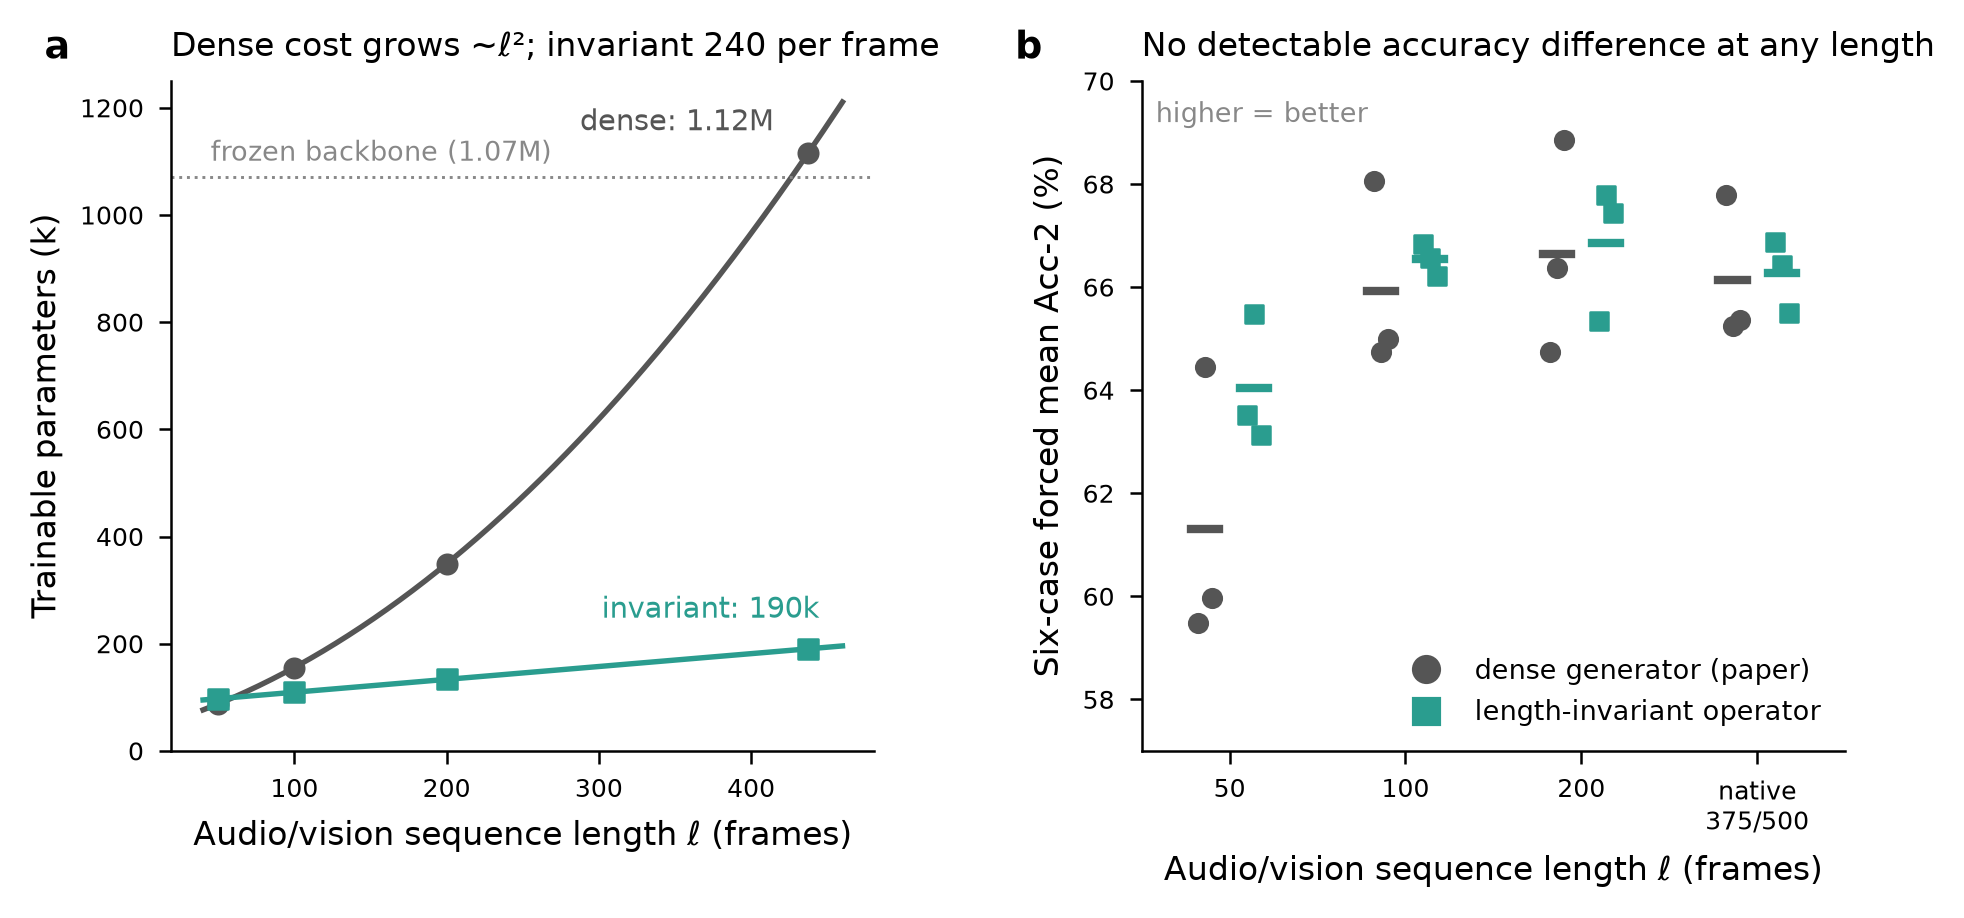
\includegraphics[width=0.92\textwidth]{fig_scaling_ladder}
\caption{(a) Trainable parameters versus audio/vision length: dense grows as $\sim\ell^2$ and exceeds the frozen backbone at native length, while the invariant operator grows by 240 parameters per frame (exact fit). (b) Six-case forced mean Acc-2 per seed, $n=3$ per arm per rung, on one machine; native uses commit \texttt{f3cebe4}. Bars are arm means.}
\label{fig:ladder}
\end{figure*}

\begin{table}[!t]
\caption{Six-case forced mean Acc-2 (\%), mean $\pm$ SD over 3 seeds; $p$ is the exact two-sided permutation test (Welch for $\ell\le200$).\label{tab:ladder}}
\centering
\setlength{\tabcolsep}{3.5pt}
\begin{tabular}{lrrrr}
\toprule
rung & dense & invariant & B$-$A & $p$\\
\midrule
$\ell=50$ & 61.30 $\pm$ 2.75 & 64.04 $\pm$ 1.25 & +2.74 & 0.22\\
$\ell=100$ & 65.93 $\pm$ 1.85 & 66.54 $\pm$ 0.32 & +0.61 & 0.63\\
$\ell=200$ & 66.65 $\pm$ 2.07 & 66.85 $\pm$ 1.32 & +0.20 & 0.89\\
native (box) & 66.13 $\pm$ 1.43 & 66.27 $\pm$ 0.70 & +0.14 & 0.80\\
native (2nd machine) & 66.01 $\pm$ 1.58 & 65.94 $\pm$ 0.75 & $-$0.08 & 0.94\\
\midrule
\multicolumn{5}{p{0.92\columnwidth}}{pooled native, machine-blocked: +0.04, 90\% CI [$-$1.59, +1.67], TOST $p=0.033$}\\
\bottomrule
\end{tabular}
\end{table}

\begin{figure*}[!t]
\centering
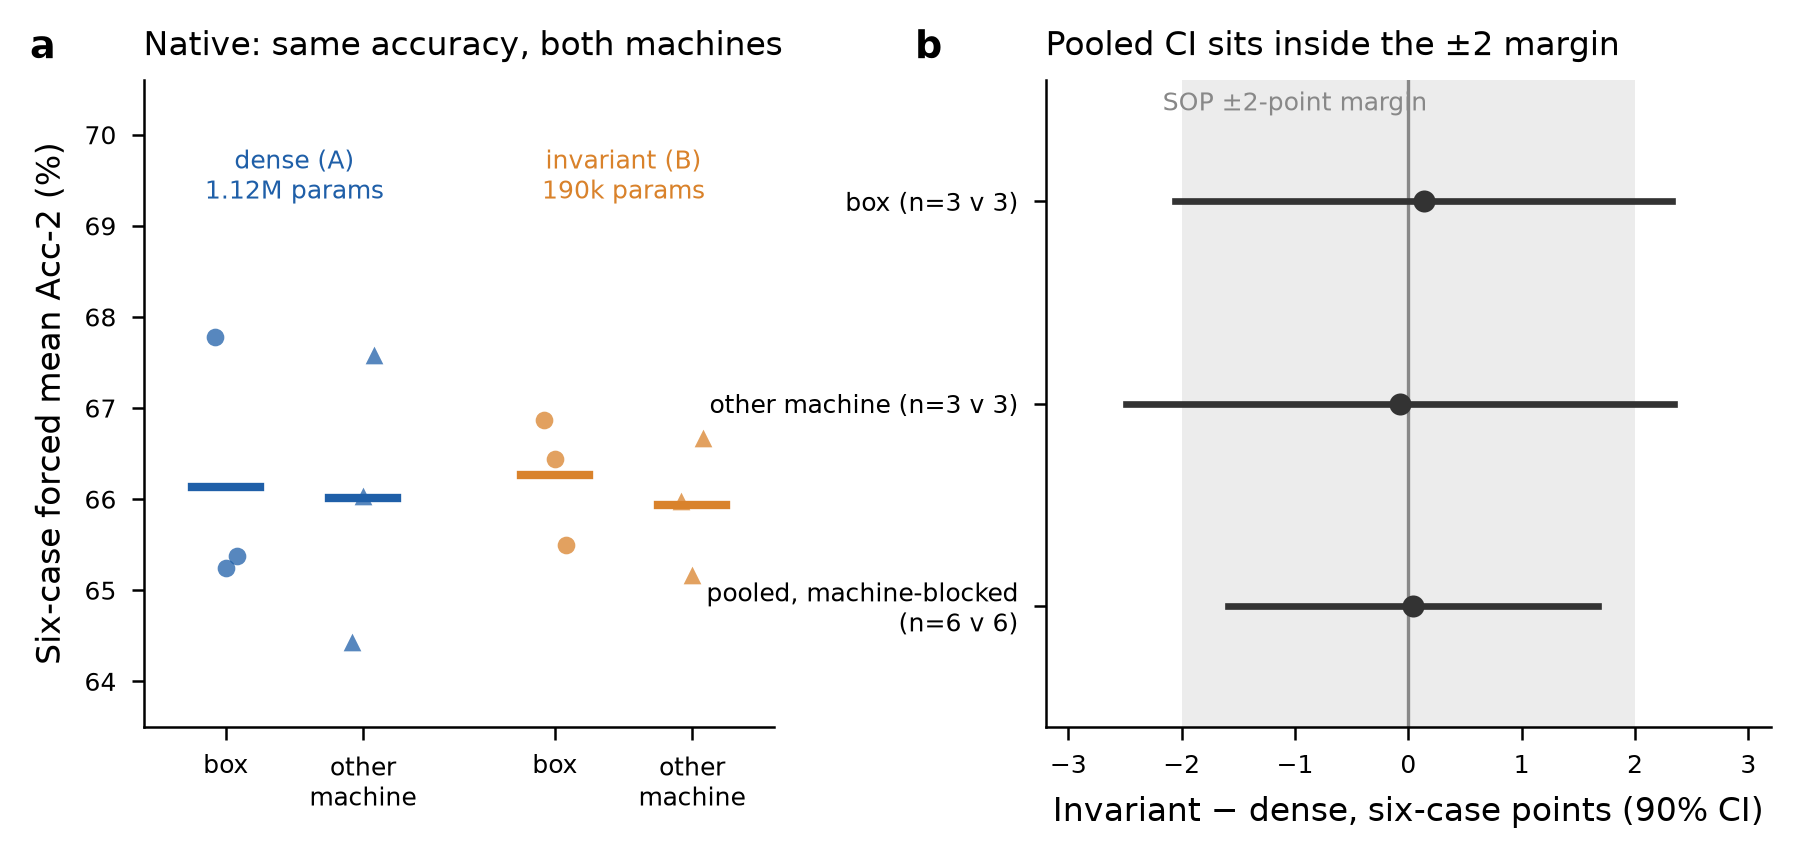
\includegraphics[width=0.85\textwidth]{native_two_machine}
\caption{Native length (375/500), $n=3$ per arm per machine. (a) Per-seed accuracy on two independent machines. (b) Invariant $-$ dense with 90\% confidence intervals; only the machine-blocked pool sits inside the SOP's $\pm$2-point equivalence margin.}
\label{fig:native}
\end{figure*}

\textbf{Our robustness prediction was wrong.} The SOP predicted that dense would degrade at long lengths. It does not. Both arms \emph{improve} by about +2.0 points per doubling over $\ell=50$--200 (OLS $p=0.0018$, $n=18$), and dense at native (66.13) is level with $\ell=200$ (66.65). The efficiency argument survives; the robustness argument does not. Inter-modal coupling stays flat along the ladder, so this is a length result, although longer rungs also mean less pooling.

\textbf{Noise floor.} The native seed-1 configuration was run three times with no seed change: on the box at commit \texttt{ebbcb4e}, on the box at \texttt{f3cebe4}, and on the second machine. This gives dense 68.57 / 67.78 / 67.58 and invariant 66.41 / 66.87 / 66.67. The three runs span commits and machines, so they bound the combined spread at about 1 point rather than isolating GPU nondeterminism. Single-run gaps under about 1 point are not interpretable.

\textbf{The $\ell=50$ complete-data inversion.} In 3 of 6 $\ell=50$ runs, complete-data accuracy is more than 2 points below the text-present missing cases (dense seed 1: 66.01 vs 70.73; invariant seeds 1 and 3: 63.26 vs 75.05 and 63.57 vs 74.49). Every $\ell=100$, 200 and native run is within 1.2 points. This is not a new anomaly. Our ledger (CLAIMS \S4.10) attributes the same inversion, seen earlier on undertrained checkpoints, to undertraining. It is confined to the cell where our loop trails the upstream loop by 7.6 points, and the upstream $\ell=50$ run shows no inversion (77.13 vs 77.08). Best epochs here (69--169) lie inside the 200-epoch budget, so if this is undertraining, the cause is the loop at this rung rather than the epoch cap. We have not tested that on these checkpoints.

\subsection{Generation fidelity is mostly padding layout}
Fig.~\ref{fig:fid} and Table~\ref{tab:fid} show the fidelity audit. MOSI audio/vision is 86--90\% left-padding, and the number of real frames (clip duration) is shared across modalities, with valid-frame counts correlated at $r=0.992$--$0.998$. Two consequences follow:
\begin{itemize}
\item The SOP's literal ``mean-pooled'' coupling measure gives about 0.53 at every rung, about 14$\times$ the real-frame value.
\item The logged time-flattened CKA rewards reproducing \emph{where the padding is}. On real frames, the dense advantage for audio/vision is not distinguishable from zero.
\end{itemize}
For text, dense is geometrically closer to the real features, yet the invariant operator's generated text carries more sentiment. Neither carries much: at most 28\% of the real text's sentiment correlation. No CKA variant predicts accuracy: Spearman $\rho=-0.005$, $-0.138$ and $-0.014$ for the logged, masked and debiased variants over 20 runs. The logged dense advantage does replicate across independent run sets: 1.84$\times$ in the 14 forty-epoch pilot runs (0.3010 vs 0.1632) and 2.16$\times$ in the 18 converged runs (0.318 vs 0.147). A replicated padding artefact, however, is still not evidence of fidelity.

\begin{table}[!t]
\caption{Fidelity of generated features, length ladder $\ell\le200$, 9 runs per arm (Welch $p$).\label{tab:fid}}
\centering
\resizebox{\columnwidth}{!}{%
\begin{tabular}{lrrr}
\toprule
measure & dense & invariant & $p$\\
\midrule
a/v CKA as logged (time-flattened) & 0.318 & 0.147 & $<$0.001\\
a/v CKA, real frames only & 0.028 & 0.022 & 0.35\\
a/v CKA vs.\ 0/1 padding mask & 0.578 & 0.249 & $<$0.001\\
text CKA, real frames & 0.109 & 0.021 & $<$0.001\\
text sentiment carried ($r$) & 0.086 & 0.158 & 0.005\\
\quad reference: real text & 0.562 & 0.560 & 0.82\\
\bottomrule
\end{tabular}}
\end{table}

\begin{figure*}[!t]
\centering
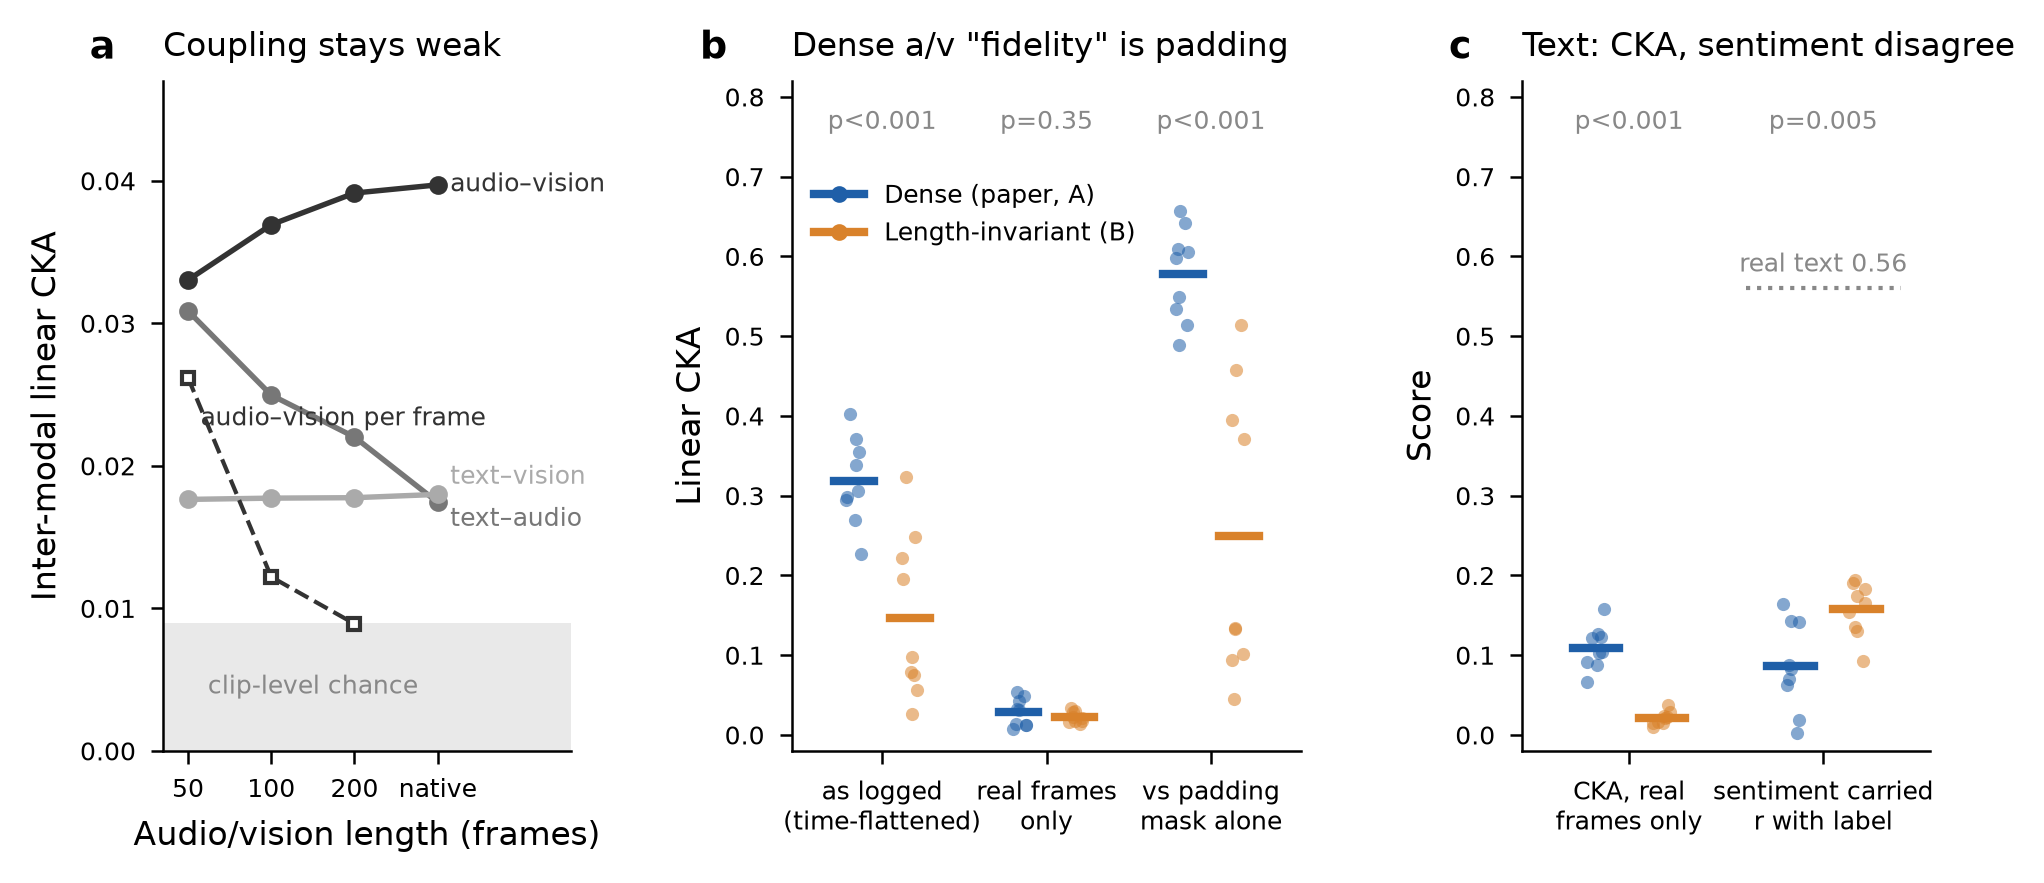
\includegraphics[width=0.95\textwidth]{ash_eval_figure}
\caption{(a) Inter-modal linear CKA along the pooled ladder (masked, z-scored, clip-level; grey band = 95th percentile of a permutation null): coupling is weak at every length. (b) Generated-vs-real audio/vision fidelity: the logged advantage of dense disappears on real frames, and dense instead reproduces the padding mask. (c) Generated text: geometric fidelity and sentiment content disagree. Nine runs per arm ($\ell=50/100/200$ $\times$ 3 seeds).}
\label{fig:fid}
\end{figure*}

\subsection{A synthetic ``L2'' rung is a noise stressor, not foundation features}\label{sec:l2syn}
The L2/L2$'$ files we first used for SOP Q2 contain no foundation-model features. They take the L1 COVAREP/Facet features, rotate them into 768/512 dimensions with random orthonormal bases, and add temporally smoothed Gaussian noise (std 0.8) in the orthogonal complement. The builder labelled them ``wav2vec2'' and ``CLIP''; we corrected the labels and treat the rung only as a controlled stressor.

Under that stressor the invariant operator degrades less than dense: 58.41 $\pm$ 0.62 vs 54.54 $\pm$ 0.33. That is +3.87, with complete rank separation, exact $p=0.10$ (the $n=3$ floor), and 2.0$\times$ the precision floor. The coupling ``gate'' originally computed for these files was itself a padding artefact. Its L1 values of 0.496 / 0.678 (audio--text / vision--text) fall to 0.023 / 0.031 on real frames, so the original gate reading is retracted.

\subsection{Real CLIP features from raw MOSI video}\label{sec:clip}
\textbf{Extraction and verification.}
\begin{itemize}
\item All 2,199 clips were extracted in 1,079~s with 0 failures.
\item On a real 640$\times$360 frame, the extractor matches reference CLIP \texttt{encode\_image} at cosine 0.99886.
\item Zero-shot, 2,198 of 2,199 middle frames are classified as ``a photo of a person talking to the camera''.
\item A ``happy person'' minus ``sad person'' prompt score correlates with the test sentiment label at $r=0.166$ ($p=1.2\times10^{-5}$).
\end{itemize}

\textbf{CLIP features are mostly speaker identity} (Fig.~\ref{fig:clip}a). 92.7\% of clip-level CLIP variance lies between speakers, against 62.8\% for Facet, 40.5\% for COVAREP and 11.1\% for GloVe. A raw ridge probe on CLIP therefore transfers nothing to unseen speakers (test $r=-0.004$, 95\% CI $[-0.074, 0.070]$), while Facet gives 0.178. After per-speaker centring, CLIP gives 0.072 and Facet 0.032. The confidence intervals overlap, so this comparison is descriptive.

\textbf{Real CLIP vision is not less correlated with the text than Facet} (Fig.~\ref{fig:clip}b). Most raw vision--audio coupling is shared speaker identity: after per-speaker centring, the excess over a within-video null falls from 0.185 to 0.003 for CLIP ($p=0.10$) and from 0.092 to $-0.001$ for Facet ($p=0.65$). Vision--text coupling survives centring for both and is slightly higher for CLIP: 0.020 vs 0.014, both $p=0.002$. This directly tests the premise of the paper's Limitations section on real foundation features, and for vision the premise is not supported.

\textbf{No detectable accuracy change} (Table~\ref{tab:clip}, Fig.~\ref{fig:clip}c). Replacing Facet with real CLIP vision changes the dense arm by $-0.93$ points ($p=0.6$) at 512 dimensions and $-0.35$ ($p=0.9$) at 20 dimensions with the label-free PCA projection. Invariant $-$ dense is null at every CLIP rung. The +3.87 synthetic-L2 advantage therefore does \emph{not} replicate on real features. Best epochs come earlier on CLIP (about 27 vs 45--53 at L1), consistent with the speaker signal being fitted quickly.

\begin{table}[!t]
\caption{Real-CLIP rungs: six-case forced mean Acc-2 (\%), mean $\pm$ SD over 3 seeds; one commit (\texttt{85eddde}), complete-data validation. $p$ is the exact permutation test.\label{tab:clip}}
\centering
\setlength{\tabcolsep}{4pt}
\resizebox{\columnwidth}{!}{%
\begin{tabular}{llrrr}
\toprule
rung & vision & dense & invariant & B$-$A ($p$)\\
\midrule
L1 & Facet 20-d & 61.96 $\pm$ 2.15 & 63.51 $\pm$ 1.15 & +1.55 (0.5)\\
L2-CLIP & CLIP 512-d & 61.03 $\pm$ 2.25 & 59.73 $\pm$ 5.09 & $-$1.30 (0.8)\\
L2$'$-CLIP & PCA-20 & 61.61 $\pm$ 6.10 & 61.95 $\pm$ 3.28 & +0.34 (0.9)\\
\midrule
\multicolumn{5}{l}{\emph{invalid control (label-aware projection, Section~\ref{sec:ablation})}}\\
L2$'$-CLIP & PLS-20 & 42.68 $\pm$ 0.79 & 48.64 $\pm$ 8.87 & --\\
L2$'$-CLIP & PLS-20, rescaled & 49.34 $\pm$ 8.62 & 48.72 $\pm$ 6.11 & $-$0.62 (1.0)\\
\bottomrule
\end{tabular}}
\end{table}

\begin{figure*}[!t]
\centering
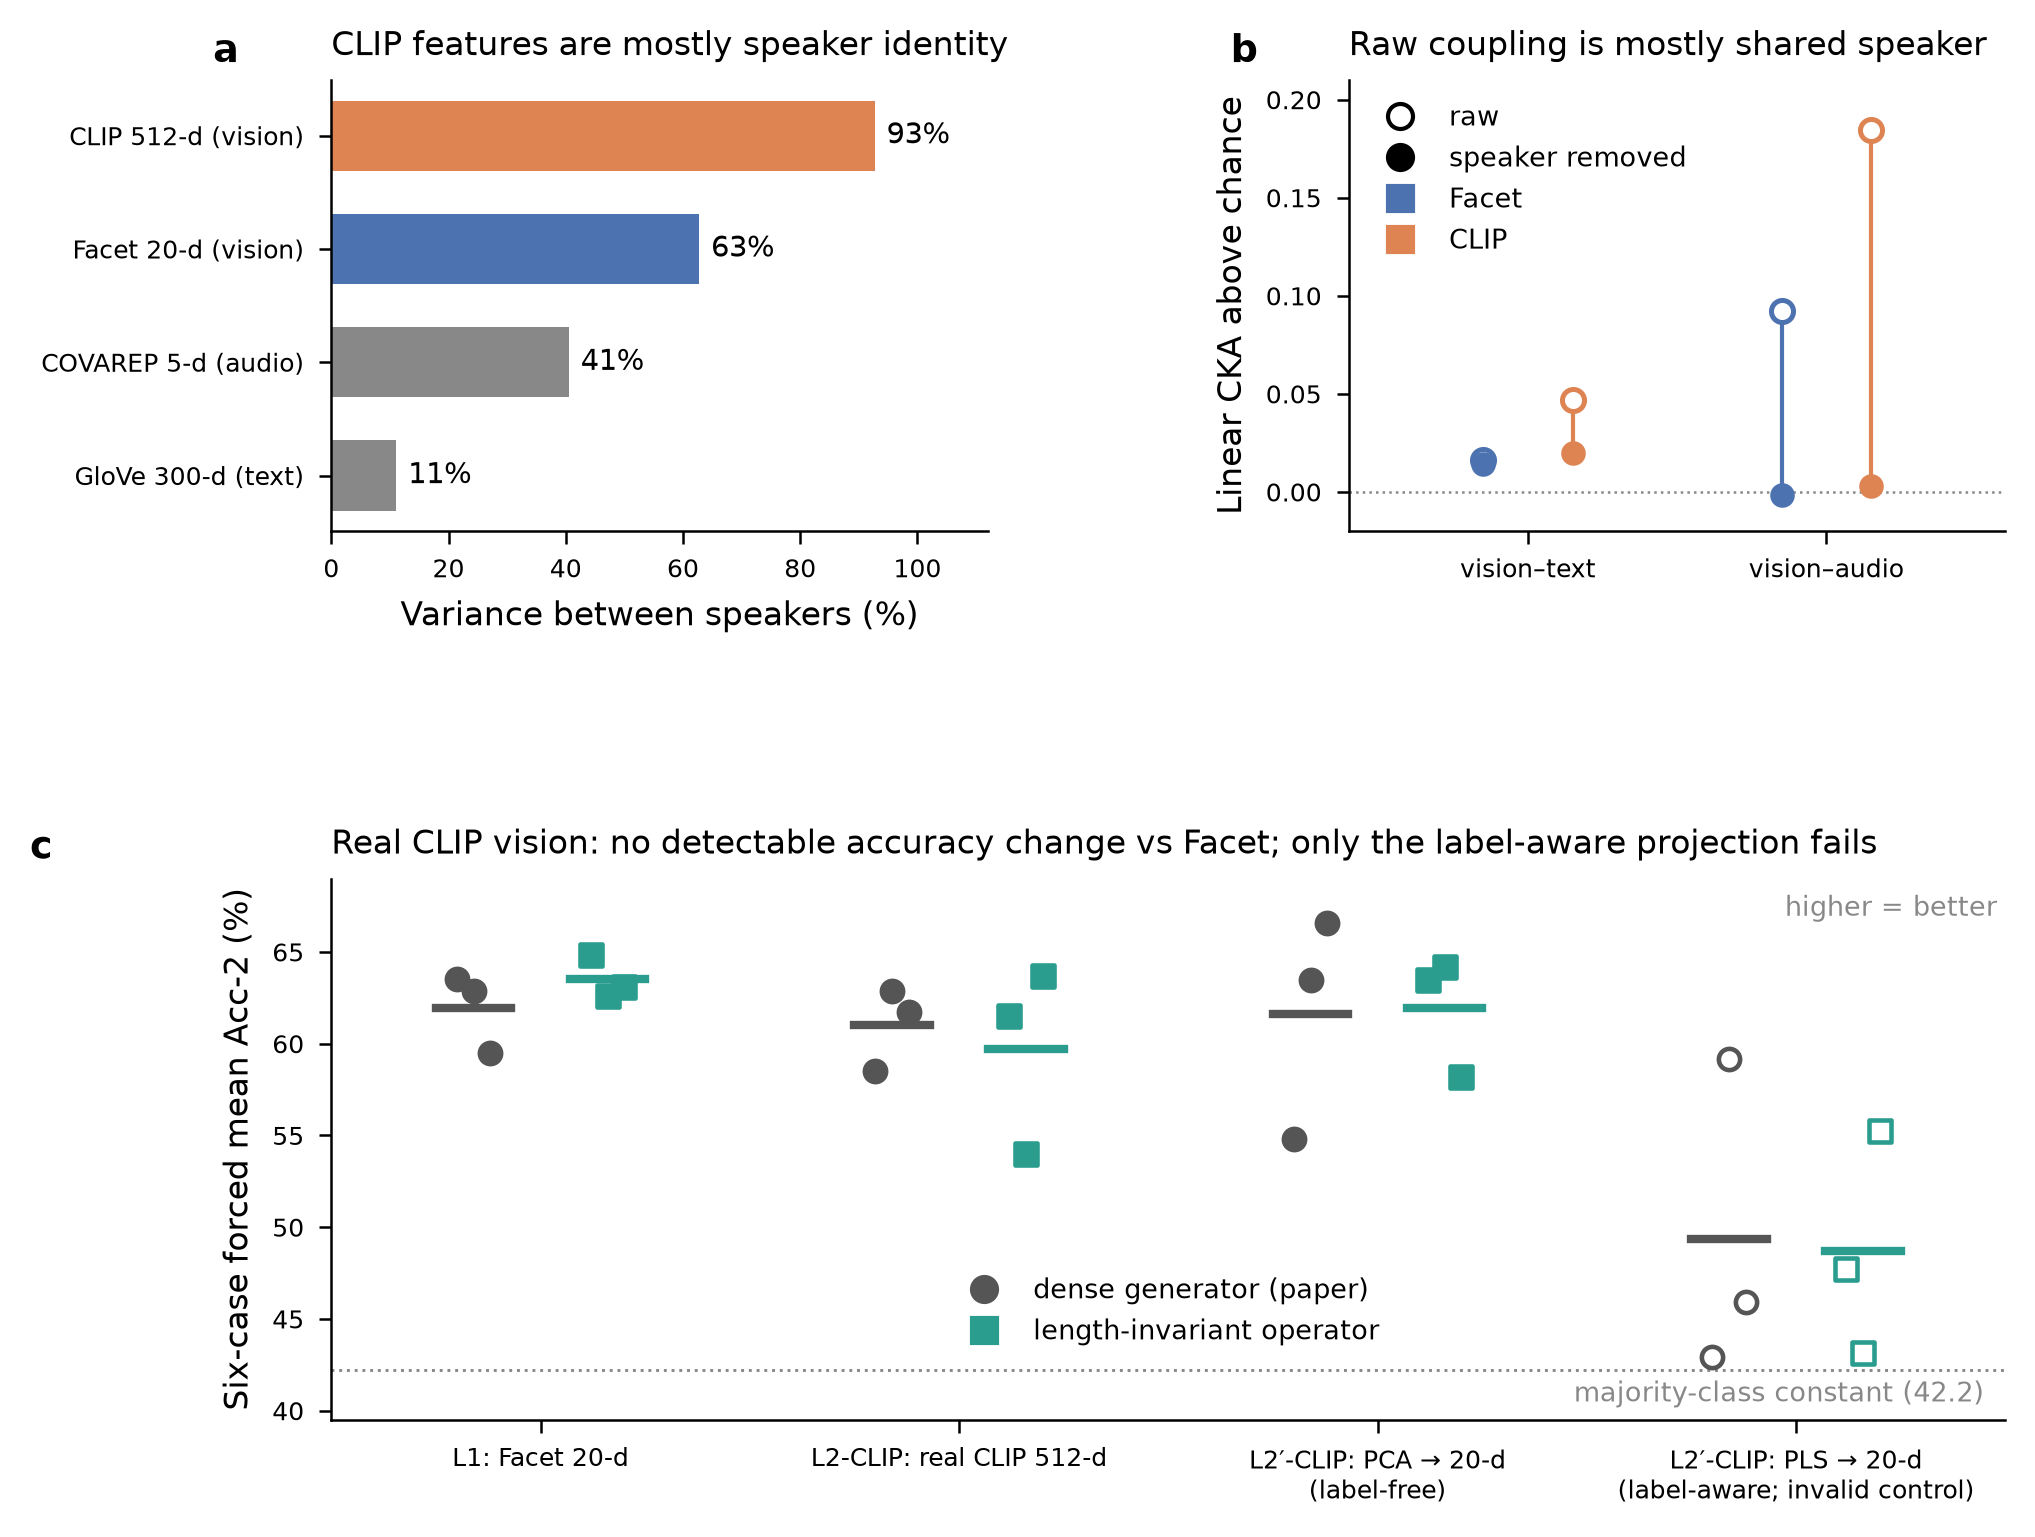
\includegraphics[width=0.85\textwidth]{clip_rungs_figure}
\caption{Real CLIP ViT-B/32 features extracted from all 2,199 raw CMU-MOSI clips. (a) Share of clip-level variance between speakers (test split, 31 speakers). (b) Inter-modal linear CKA above a permutation null, raw (hollow) and with speaker removed (filled; null permuted within video). (c) Per-seed accuracy, $n=3$ per arm; hollow markers mark the label-aware PLS rung, an invalid control. The first, unscaled PLS build is listed in Table~\ref{tab:clip} but not plotted.}
\label{fig:clip}
\end{figure*}

\section{Ablation Study}\label{sec:ablation}
\subsection{Is the learned time-mixing layer needed? (arms C, D)}
At $\ell=200$ (Fig.~\ref{fig:arms}) the four arms score:
\begin{itemize}
\item A, dense (paper): 66.65 $\pm$ 2.07;
\item B, invariant: 66.85 $\pm$ 1.32;
\item C, dense frozen at random initialisation: 65.15 $\pm$ 0.52;
\item D, zero-parameter fixed pool: 66.98 $\pm$ 0.79.
\end{itemize}
No arm differs from A: one-way ANOVA $F=1.25$, $p=0.354$. Deleting the 262,950 learned time-mixing parameters (D vs A) changes accuracy by +0.33 (Welch $p=0.82$, 90\% CI $[-2.90, +3.56]$). On the paper's extracted features, the learned time-mixing layer buys no detectable accuracy. The fidelity audit points the same way. Logged audio/vision CKA is 0.292 for trained dense, 0.289 for random-frozen dense and 0.298 for the fixed pool, and all three match the padding mask equally (0.54--0.59). The logged metric therefore cannot distinguish a trained generator from an untrained one. Descriptively, D exceeds C by +1.83 (Welch $t=3.37$, $p=0.035$), and C's deficit is confined to text-absent cases (52.41 vs 55.45 for A; text-present 77.90 vs 77.85), consistent with A4's larger deficit where text is absent. This is one of several pairwise comparisons under a null omnibus test and does not survive Holm correction. Arm D selects late (best epochs 197, 132 and 158), so 200 epochs may still truncate it. Arms C and D ran at project commit \texttt{73a2769} and arms A and B at \texttt{ebbcb4e}. The intervening edits are additive, but the comparison departs from our one-commit rule.

\begin{figure*}[!t]
\centering
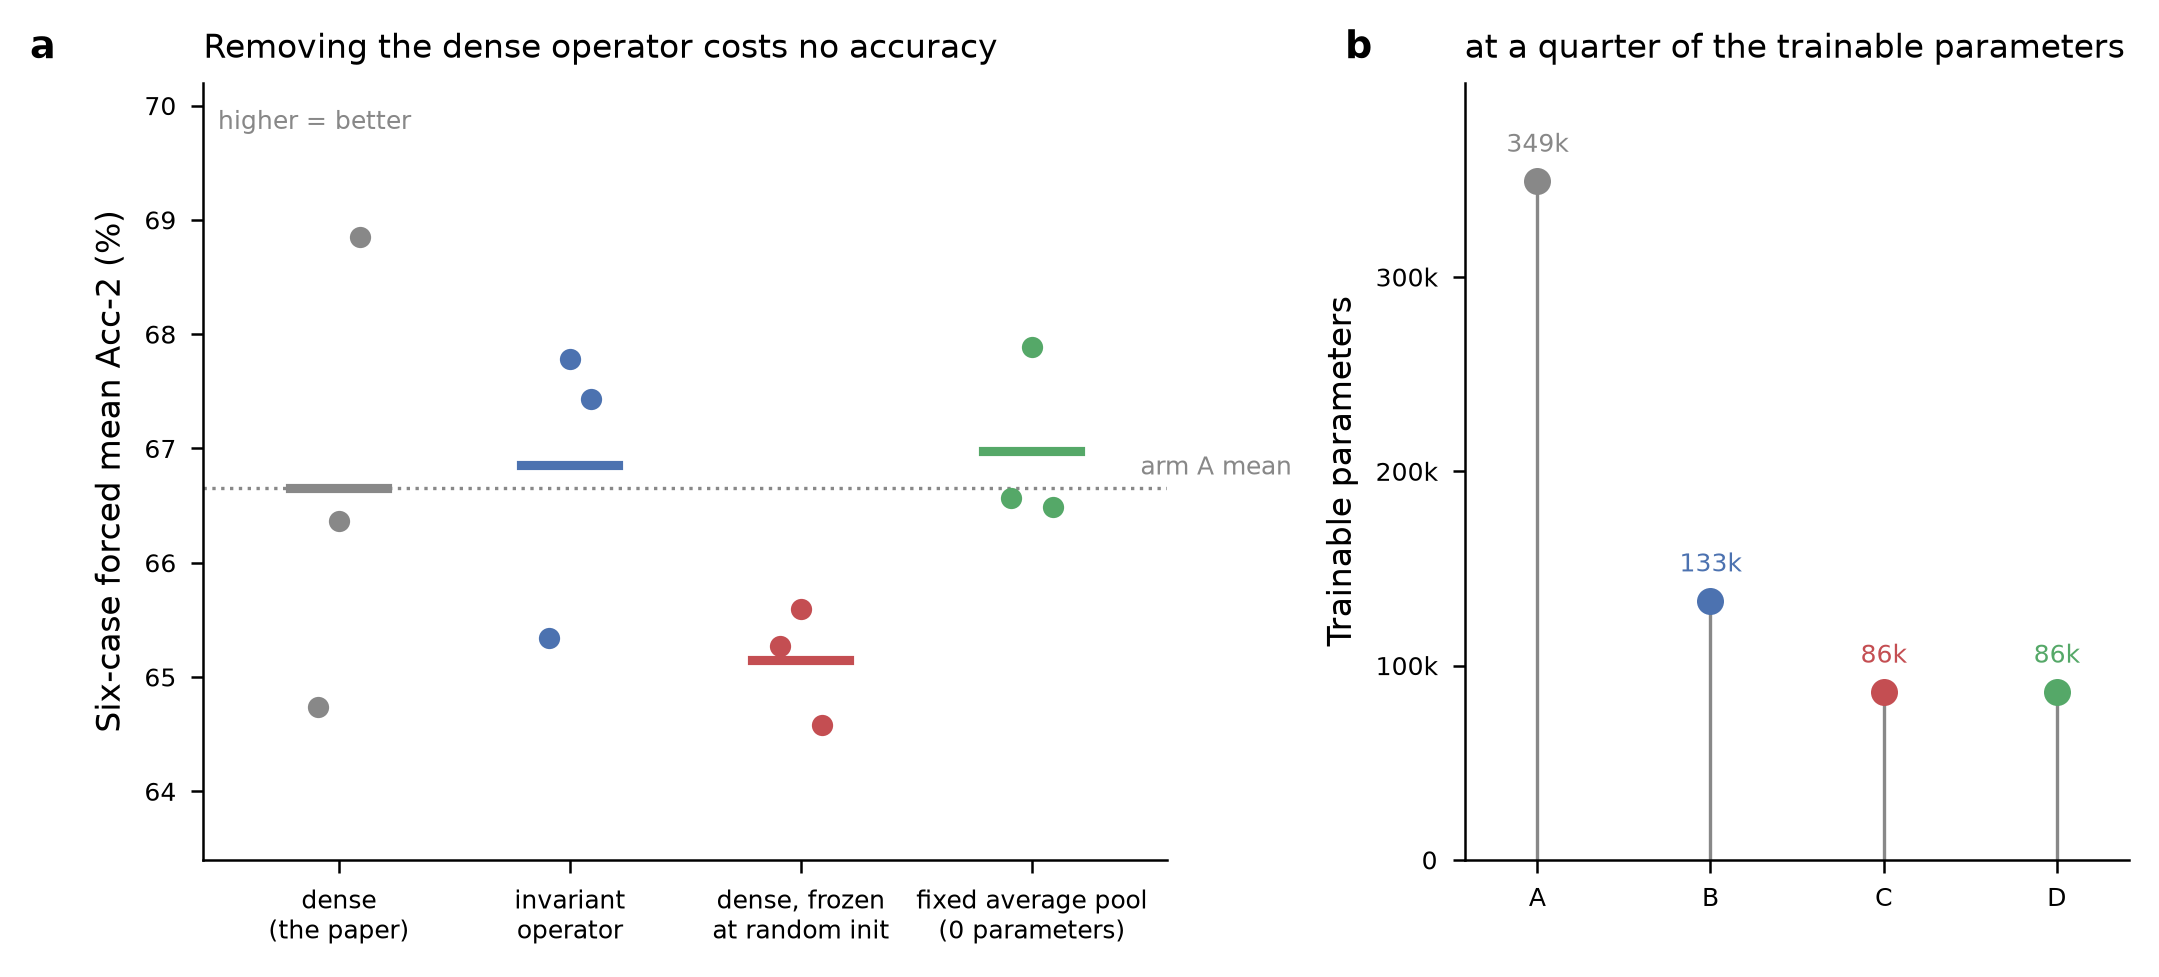
\includegraphics[width=0.85\textwidth]{arms_abcd_l200}
\caption{Operator ablation at $\ell=200$, $n=3$ per arm, one machine. (a) Six-case forced mean Acc-2 per seed; dotted line = arm A mean. (b) Trainable parameters. Arms C and D train the identical 86,491-parameter set; C keeps 262,950 dense time-mixing weights frozen at random initialisation, and D removes them.}
\label{fig:arms}
\end{figure*}

\textbf{Boundary.} Under the synthetic noise stressor, the same ablation does cost accuracy. Dense scores 54.54, against C 52.63 and D 52.49, and all six C/D runs fall below every dense run. That gap is only 1.0--1.1$\times$ the precision floor, so it is not established. The claim is therefore bounded: \emph{on the paper's features}, the learned time-mixer is unnecessary.

\subsection{Label-aware versus label-free projection}
The SOP's L2$'$ control projects high-dimensional features to Facet's 20 dimensions with PLS fitted on the training labels. On MOSI this is invalid (Table~\ref{tab:pls}). Because the splits are speaker-independent, PLS memorises each \emph{training speaker's} average sentiment, and that does not transfer to unseen speakers. The model takes this shortcut and ignores the text: text-present cases drop 18--25 points. The PLS scores were also about 13$\times$ Facet's scale. Unscaled, all three dense seeds sat at the 42.23\% majority-class constant (best epochs 1--2); rescaling removed the constant but not the failure. A label-free PCA projection at the same dimension and scale trains normally (61.61 / 61.95). The synthetic L2$'$ rung shares the flaw, which plausibly explains its unstable seeds.

\begin{table}[!t]
\caption{Linear fit of clip-level vision features to the label (fitted on train).\label{tab:pls}}
\centering
\setlength{\tabcolsep}{4pt}
\resizebox{\columnwidth}{!}{%
\begin{tabular}{lrrrr}
\toprule
features & train $r$ & valid $r$ & test $r$ & speaker-level train $r$\\
\midrule
CLIP $\rightarrow$ PLS-20 & 0.673 & 0.006 & 0.029 & \textbf{0.991}\\
synthetic L2$'$ (PLS-20) & 0.671 & $-$0.054 & 0.068 & \textbf{0.911}\\
CLIP $\rightarrow$ PCA-20 & 0.345 & 0.200 & 0.053 & --\\
Facet 20-d (L1) & 0.341 & 0.237 & 0.178 & 0.615\\
\bottomrule
\end{tabular}}
\end{table}

\subsection{Checkpoint-selection protocol and training budget}
\textbf{Checkpoint selection.} Selecting on complete-data rather than dropout-0.7 validation stabilised the synthetic-L2 arms. Dense went from 54.01 $\pm$ 1.07 to 54.54 $\pm$ 0.33, and invariant from 56.90 $\pm$ 0.81 to 58.41 $\pm$ 0.62. It did not rescue L2$'$: it changed which seed collapsed.

\textbf{Training budget.} Training for 200 rather than 40 epochs changed the six-case mean by only +0.67 points across 14 seed-matched cells ($p=0.17$). This retracts an earlier claim that 40 epochs cost about 7 points. That claim set a 40-epoch run of our loop (61.89) against a 200-epoch run of the upstream loop (68.93), so most of its ``7 points'' is the loop gap of Section~\ref{sec:loops}. The pilot's asymmetric-truncation hypothesis also failed. Invariant runs had peaked later at 40 epochs (mean best epoch 35.0 vs 27.3), which predicted that more budget would favour the invariant arm. Instead, 200 epochs moved dense by +1.27 and invariant by $-$0.52 at $\ell=100$, and by +0.75 and +0.60 over all 14 matched cells.

\textbf{Preprocessing.} Replacing the extractor's original 224$\times$224 squash with CLIP's official shorter-side resize and centre crop raised agreement with reference CLIP on 4:3 frames from 0.951--0.986 to 0.999.

\section{Discussion}
\textbf{Fault in the paper, or in the code?} \emph{In the code} --- proven:
\begin{itemize}
\item one prompt type is structurally untrainable (A3);
\item the evaluation reports the wrong split and the defaults undertrain (A4);
\item the module's cost scales with length in a way the paper does not disclose (A1);
\item the released code does not install from its stated requirements or load its own checkpoints on current PyTorch (A5).
\end{itemize}
Each fault, its location and a proposed fix are collected in Table~\ref{tab:faults} and in a separate correction note addressed to the authors.
We did \emph{not} show that the paper's 72.14\% is wrong; the remaining 4.63-point gap is open. The defensible claim is: \emph{the released implementation cannot reproduce the paper's ablations, and its generation module's learned, length-bound parameters can be replaced or removed at no detectable accuracy cost.}

\textbf{Why does generation matter so little?} Three lines of evidence agree:
\begin{enumerate}
\item the time-mixer can be deleted (arm D) at no detectable cost;
\item its ``reconstruction'' mostly reproduces padding layout;
\item what it generates carries at most a quarter of the real text's sentiment signal, and essentially none of the real audio/vision signal.
\end{enumerate}
Text dominates MOSI: GloVe alone gives a probe $r$ of 0.58, against 0.18--0.24 for Facet and COVAREP. So the benefit of the module is small wherever text is present.

\textbf{SOP Table~III reading.} For vision on real CLIP features, accuracy and real-frame fidelity are both stable: masked a/v CKA for the dense arm is 0.026 at L1 and 0.026 at L2-CLIP, and inter-modal coupling is not lower. This matches the row ``G, A both stable $\rightarrow$ concern unfounded''. The margin $M$ over a backbone-only control was not measured.

\begin{table}[!t]
\caption{Proposed (SOP) versus delivered.\label{tab:sop}}
\centering
\setlength{\tabcolsep}{3pt}
\begin{tabular}{p{3.3cm}p{1.2cm}p{3.5cm}}
\toprule
commitment & status & evidence\\
\midrule
Q1 structural scaling & yes & Tab.~\ref{tab:params}, A2\\
Dead-prompt repair & mechanism & A3; accuracy not measured\\
Reproduction gate (72.14 $\pm$ 2) & missed & 67.51; causes located (A4)\\
Q2 length ladder & yes & Fig.~\ref{fig:ladder}; prediction refuted\\
Q2 features / correlation & vision only & real CLIP rungs (Sec.~\ref{sec:clip})\\
Q3 length-invariant operator & yes & equivalence at native\\
Operator ablations & partly & arms C, D; no strided/dilated conv\\
Fidelity $G$ (primary) & corrected & audit, Tab.~\ref{tab:fid}\\
Margin $M$ (primary) & no & no backbone-only control\\
CLIP extractor + merge & yes & 2,199 clips, verified\\
5 seeds & 3 seeds & pre-registered fallback\\
\bottomrule
\end{tabular}
\end{table}

\section{Limitations}
\begin{itemize}
\item \textbf{Reproduction gap.} The 4.63-point gap to the paper is unexplained, and the corrected baseline rests on one seed.
\item \textbf{Modalities.} Only vision was replaced by a foundation feature; audio stays COVAREP, so the real-CLIP rungs mix feature pipelines. The frozen backbone was pre-trained on Facet-style MOSEI features, so only the input projection adapts to CLIP.
\item \textbf{Statistical power.} With $n=3$ seeds, most results are ``no detectable difference''. Equivalence is shown only at native length and only on the two-machine pool; at $\ell=200$, about 14 seeds per arm would be needed.
\item \textbf{Scope.} CMU-MOSI only; no CMU-MOSEI fine-tuning, CH-SIMS or IEMOCAP.
\item \textbf{Repair cost.} The invariant operator is 12.5\% of the backbone at $\ell=200$ and 17.8\% at native, above the paper's 5--10\% envelope, and slightly larger than dense below 60 frames. The claim is ``5.86$\times$ cheaper than dense'', not ``within budget''.
\item \textbf{$\ell=50$ inversion.} Linked to undertraining and to the loop gap (Section~\ref{sec:results}), but not tested on these checkpoints.
\item \textbf{Two loops.} The 7.6-point gap between the upstream loop and ours is measured on one cell, against one upstream run whose seed and dropout are unrecorded; its cause is not isolated. A4 and the end-term grids are not comparable.
\item \textbf{Repair untrained.} The dead-prompt repair is verified mechanically, not trained to convergence; its expected effect (about 0.2 points) is below our precision floor.
\item \textbf{Locality scope.} A2's diagonal-mass test cannot detect non-local temporal structure; the SVD/row-similarity check is not done.
\item \textbf{Protocol differences.} The ladder (dropout-0.7 selection) and the CLIP grids (complete-data selection) use different checkpoint-selection protocols. Our loop is not bit-reproducible, and arms C/D ran at a different commit from arms A/B.
\item \textbf{Layout approximation.} The CLIP word-slot layout uses a uniform split of each clip, not word timestamps; agreement with Facet's slots is 99.1--99.5\%.
\end{itemize}

\section{Conclusion and Future Work}
MPLMM's released generation module is neither as light nor as necessary as presented. Its time-mixing layer grows with sequence length past the size of the frozen backbone, one of its three prompt types never trains (a one-line re-initialisation revives it), its evaluation reports the wrong split under randomly corrupted inputs, and it does not run on current PyTorch without patches. Its training loop and our fork's loop are not interchangeable, so every comparison here stays inside one loop. Replacing the time-mixer with a length-invariant operator preserves accuracy at every length and is equivalent at native length with 5.86$\times$ fewer parameters. Deleting the learned time-mixer costs no detectable accuracy on the paper's features. On real CLIP features extracted from the raw MOSI video, the failure the authors predicted does not appear for vision, and the weaker cross-modal correlation it rests on is not observed.

\textbf{Future work:}
\begin{itemize}
\item extract wav2vec~2.0 audio to complete the foundation-feature rung;
\item add backbone-only and generator-bypassed controls to measure the margin $M$;
\item use speaker-grouped cross-fitting for any label-aware projection;
\item raise seeds to establish equivalence at $\ell\le200$;
\item test on MOSEI and CH-SIMS;
\item train the repaired missing-type prompt to convergence;
\item run the upstream and fork loops on one cell with matched seed and dropout to isolate the 7.6-point gap;
\item run the SVD/row-similarity check that closes A2's scope;
\item submit the accompanying correction note to \texttt{zrguo/MPLMM} as issues, with patches.
\end{itemize}

\bibliographystyle{IEEEtran}
\bibliography{ref}

\appendix[AI tools, prompts and verification]
The instructor permitted AI-assisted coding for this project.

\textbf{Platforms.}
\begin{itemize}
\item Claude (chat) for literature scoping and experimental design.
\item Claude Code for tracing the MPLMM, MMSA, MMSA-FET and CMU-MultimodalSDK codebases.
\item Claude Science (an agentic analysis environment with SSH access to the project GPU box) for the end-term evaluation:
  \begin{itemize}
  \item the fidelity and CKA audits and the statistics;
  \item the length-ladder, native, arm C/D and CLIP grids, driven by detached supervisors;
  \item extractor hardening and verification;
  \item figures and this report's numbers.
  \end{itemize}
\end{itemize}
Teammates' own AI usage for their components (operator, training runs, ladder resampler, extractor code) is not recorded here; each member should add theirs.

\textbf{Representative prompts} (Ash, end-term):
\begin{itemize}
\item ``What should be our end-term deliverable that will be solid considering our project status and goals, what we've proved till now, the numbers we have\ldots''
\item ``Verify the CLIP extractor is working and is well.''
\item ``Load real CMU-MOSI video and test this CLIP extractor on it; I want real results to showcase the CLIP extractor as a finding.''
\item ``Does this evaluation prove a new finding or boost our case, or should we wait for the L2$'$ results?''
\item ``Give a comprehensive project report summarising all key findings and the data behind them, following the given format.''
\end{itemize}

\textbf{Verification protocol and AI errors caught.} Every number in this report is read from a run record or results file, and every claim in the project's claims ledger carries a status tag. AI-generated errors that were caught and retracted:
\begin{itemize}
\item an inverted axis (``temporal receptive field of one position''), which reached the proposal abstract;
\item ``40 epochs cost $\sim$7 points'' (a cross-entry-point comparison);
\item a padding-inflated coupling gate (L1 CKA 0.496/0.678, real frames 0.023/0.031);
\item a Welch $p=0.002$ reported at $n=3$, where the exact floor is 0.10;
\item ``dense is best at native'';
\item a synthetic rung mislabelled as wav2vec2/CLIP features;
\item our own label-aware PLS control, which leaks training-speaker sentiment;
\item ``1.42 points of GPU nondeterminism'' (the 67.51/68.93 difference is data and loop, not noise);
\item the pilot's asymmetric-truncation hypothesis (200 epochs moved dense +1.27 and invariant $-$0.52 at $\ell=100$);
\item ``training is not bit-reproducible'' stated without scope (true of our loop only; the upstream loop is byte-identical per machine);
\item the $\ell=50$ inversion presented as a fresh, unexplained anomaly (it matches CLAIMS \S4.10).
\end{itemize}
Each correction names the superseded value so that it cannot reappear.

\end{document}
